\documentclass{standalone}
\usepackage{tikz}
\usetikzlibrary{patterns, positioning}
\usepackage[sfdefault]{ClearSans} %% option 'sfdefault' activates Clear Sans as the default text font
\usepackage[T1]{fontenc}

\begin{document}
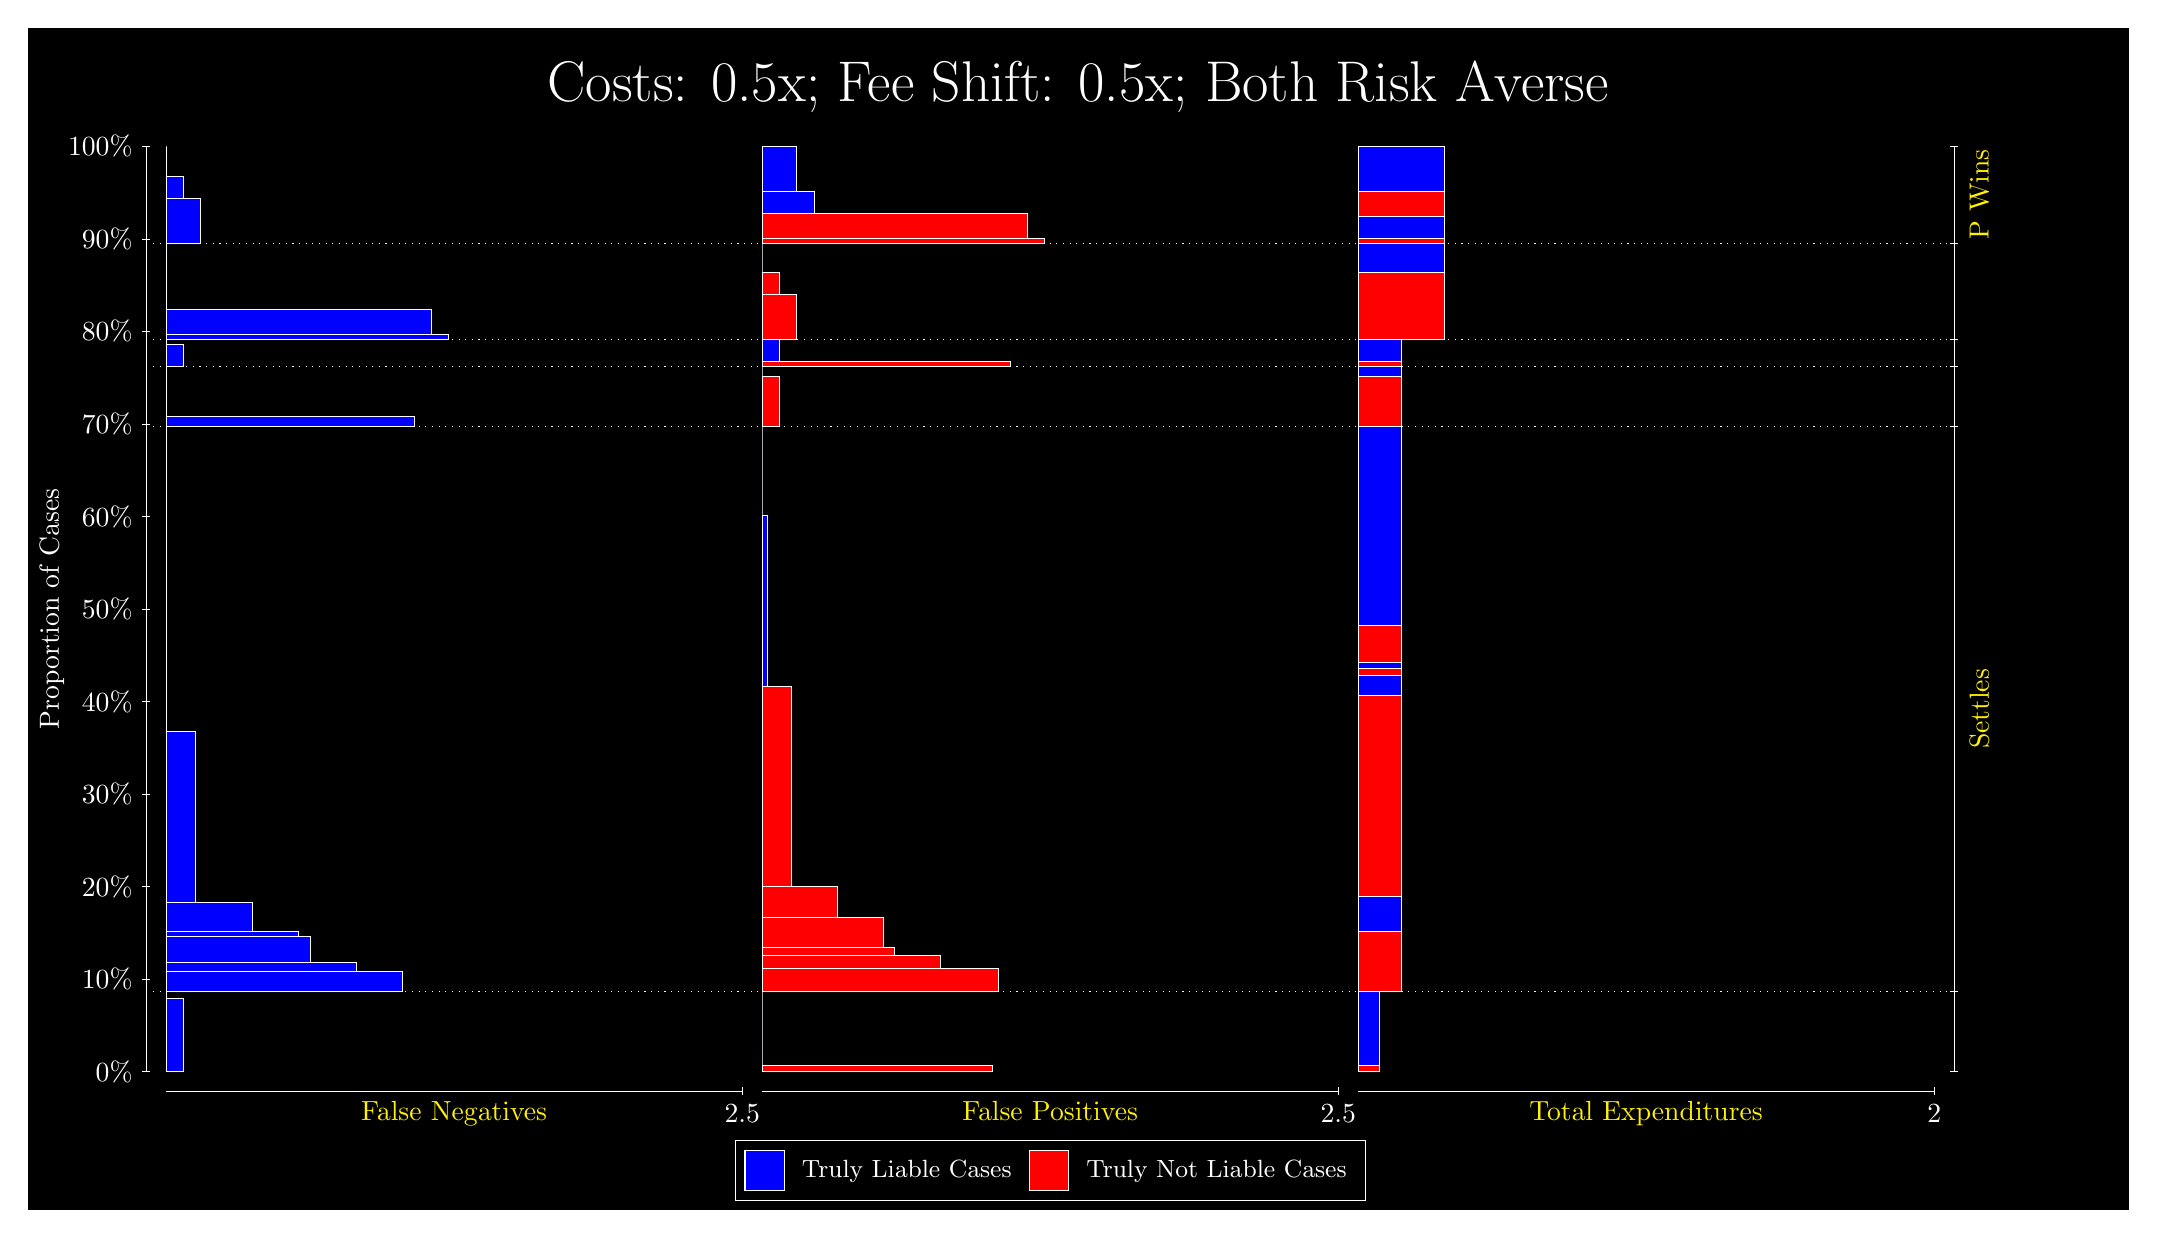
\begin{tikzpicture}
\draw[fill=black] (0,0) rectangle (26.667,15);
\draw[text=white] (0,13.5) rectangle (26.667,15) node[midway] {\huge Costs: 0.5x; Fee Shift: 0.5x; Both Risk Averse};
\draw[white, very thin] (1.5,1.75) -- (1.5,13.5);
\node[rotate=90, text=white, anchor=center] at (0.3, 7.625) {Proportion of Cases};
\draw[white, very thin] (1.45,1.75) -- (1.55,1.75);
\node[text=white, anchor=east] at (1.45, 1.75) {0\%};
\draw[white, very thin] (1.45,2.925) -- (1.55,2.925);
\node[text=white, anchor=east] at (1.45, 2.925) {10\%};
\draw[white, very thin] (1.45,4.1) -- (1.55,4.1);
\node[text=white, anchor=east] at (1.45, 4.1) {20\%};
\draw[white, very thin] (1.45,5.275) -- (1.55,5.275);
\node[text=white, anchor=east] at (1.45, 5.275) {30\%};
\draw[white, very thin] (1.45,6.45) -- (1.55,6.45);
\node[text=white, anchor=east] at (1.45, 6.45) {40\%};
\draw[white, very thin] (1.45,7.625) -- (1.55,7.625);
\node[text=white, anchor=east] at (1.45, 7.625) {50\%};
\draw[white, very thin] (1.45,8.8) -- (1.55,8.8);
\node[text=white, anchor=east] at (1.45, 8.8) {60\%};
\draw[white, very thin] (1.45,9.975) -- (1.55,9.975);
\node[text=white, anchor=east] at (1.45, 9.975) {70\%};
\draw[white, very thin] (1.45,11.15) -- (1.55,11.15);
\node[text=white, anchor=east] at (1.45, 11.15) {80\%};
\draw[white, very thin] (1.45,12.325) -- (1.55,12.325);
\node[text=white, anchor=east] at (1.45, 12.325) {90\%};
\draw[white, very thin] (1.45,13.5) -- (1.55,13.5);
\node[text=white, anchor=east] at (1.45, 13.5) {100\%};

\draw[white, very thin] (24.457,1.75) -- (24.457,13.5);
\draw[white, very thin] (24.407,1.75) -- (24.507,1.75);
\node[anchor=west] at (24.407, 1.75) {};
\draw[white, very thin] (24.407,2.7635) -- (24.507,2.7635);
\node[anchor=west] at (24.407, 2.7635) {};
\draw[white, very thin] (24.407,9.9463) -- (24.507,9.9463);
\node[anchor=west] at (24.407, 9.9463) {};
\draw[white, very thin] (24.407,10.708) -- (24.507,10.708);
\node[anchor=west] at (24.407, 10.708) {};
\draw[white, very thin] (24.407,11.052) -- (24.507,11.052);
\node[anchor=west] at (24.407, 11.052) {};
\draw[white, very thin] (24.407,12.271) -- (24.507,12.271);
\node[anchor=west] at (24.407, 12.271) {};
\draw[white, very thin] (24.407,13.5) -- (24.507,13.5);
\node[anchor=west] at (24.407, 13.5) {};

\draw[white, very thin, fill=blue] (1.75,1.75) rectangle (1.9696,2.6814);
\draw[white, very thin, fill=red] (1.75,2.6814) rectangle (1.75,2.7635);
\draw[white, very thin, fill=blue] (1.75,2.7635) rectangle (4.7507,3.02);
\draw[white, very thin, fill=blue] (1.75,3.02) rectangle (4.1652,3.1376);
\draw[white, very thin, fill=blue] (1.75,3.1376) rectangle (3.5797,3.4642);
\draw[white, very thin, fill=blue] (1.75,3.4642) rectangle (3.4333,3.5333);
\draw[white, very thin, fill=blue] (1.75,3.5333) rectangle (2.8478,3.8943);
\draw[white, very thin, fill=blue] (1.75,3.8943) rectangle (2.1159,6.0664);
\draw[white, very thin, fill=red] (1.75,6.0664) rectangle (1.75,9.9463);
\draw[white, very thin, fill=blue] (1.75,9.9463) rectangle (4.8971,10.075);
\draw[white, very thin, fill=red] (1.75,10.075) rectangle (1.75,10.708);
\draw[white, very thin, fill=blue] (1.75,10.708) rectangle (1.9696,10.991);
\draw[white, very thin, fill=red] (1.75,10.991) rectangle (1.75,11.052);
\draw[white, very thin, fill=blue] (1.75,11.052) rectangle (5.3362,11.109);
\draw[white, very thin, fill=blue] (1.75,11.109) rectangle (5.1167,11.428);
\draw[white, very thin, fill=red] (1.75,11.428) rectangle (1.75,12.271);
\draw[white, very thin, fill=blue] (1.75,12.271) rectangle (2.1891,12.841);
\draw[white, very thin, fill=blue] (1.75,12.841) rectangle (1.9696,13.124);
\draw[white, very thin, fill=red] (1.75,13.124) rectangle (1.75,13.5);
\draw[white, very thin, fill=red] (9.3189,1.75) rectangle (12.246,1.832);
\draw[white, very thin, fill=blue] (9.3189,1.832) rectangle (9.3189,2.7635);
\draw[white, very thin, fill=red] (9.3189,2.7635) rectangle (12.32,3.061);
\draw[white, very thin, fill=red] (9.3189,3.061) rectangle (11.588,3.2322);
\draw[white, very thin, fill=red] (9.3189,3.2322) rectangle (11.002,3.3268);
\draw[white, very thin, fill=red] (9.3189,3.3268) rectangle (10.856,3.7081);
\draw[white, very thin, fill=red] (9.3189,3.7081) rectangle (10.27,4.0983);
\draw[white, very thin, fill=red] (9.3189,4.0983) rectangle (9.6848,6.6433);
\draw[white, very thin, fill=blue] (9.3189,6.6433) rectangle (9.3921,8.8154);
\draw[white, very thin, fill=blue] (9.3189,8.8154) rectangle (9.3189,9.9463);
\draw[white, very thin, fill=red] (9.3189,9.9463) rectangle (9.5384,10.579);
\draw[white, very thin, fill=blue] (9.3189,10.579) rectangle (9.3189,10.708);
\draw[white, very thin, fill=red] (9.3189,10.708) rectangle (12.466,10.769);
\draw[white, very thin, fill=blue] (9.3189,10.769) rectangle (9.5384,11.052);
\draw[white, very thin, fill=red] (9.3189,11.052) rectangle (9.758,11.616);
\draw[white, very thin, fill=red] (9.3189,11.616) rectangle (9.5384,11.895);
\draw[white, very thin, fill=blue] (9.3189,11.895) rectangle (9.3189,12.271);
\draw[white, very thin, fill=red] (9.3189,12.271) rectangle (12.905,12.329);
\draw[white, very thin, fill=red] (9.3189,12.329) rectangle (12.686,12.648);
\draw[white, very thin, fill=blue] (9.3189,12.648) rectangle (9.9776,12.931);
\draw[white, very thin, fill=blue] (9.3189,12.931) rectangle (9.758,13.5);
\draw[white, very thin, fill=red] (16.888,1.75) rectangle (17.162,1.832);
\draw[white, very thin, fill=blue] (16.888,1.832) rectangle (17.162,2.7635);
\draw[white, very thin, fill=red] (16.888,2.7635) rectangle (17.437,3.535);
\draw[white, very thin, fill=blue] (16.888,3.535) rectangle (17.437,3.9793);
\draw[white, very thin, fill=red] (16.888,3.9793) rectangle (17.437,6.5243);
\draw[white, very thin, fill=blue] (16.888,6.5243) rectangle (17.437,6.7807);
\draw[white, very thin, fill=red] (16.888,6.7807) rectangle (17.437,6.8753);
\draw[white, very thin, fill=blue] (16.888,6.8753) rectangle (17.437,6.9444);
\draw[white, very thin, fill=red] (16.888,6.9444) rectangle (17.437,7.4131);
\draw[white, very thin, fill=blue] (16.888,7.4131) rectangle (17.437,9.9463);
\draw[white, very thin, fill=red] (16.888,9.9463) rectangle (17.437,10.579);
\draw[white, very thin, fill=blue] (16.888,10.579) rectangle (17.437,10.708);
\draw[white, very thin, fill=red] (16.888,10.708) rectangle (17.437,10.769);
\draw[white, very thin, fill=blue] (16.888,10.769) rectangle (17.437,11.052);
\draw[white, very thin, fill=red] (16.888,11.052) rectangle (17.986,11.895);
\draw[white, very thin, fill=blue] (16.888,11.895) rectangle (17.986,12.271);
\draw[white, very thin, fill=red] (16.888,12.271) rectangle (17.986,12.329);
\draw[white, very thin, fill=blue] (16.888,12.329) rectangle (17.986,12.612);
\draw[white, very thin, fill=red] (16.888,12.612) rectangle (17.986,12.931);
\draw[white, very thin, fill=blue] (16.888,12.931) rectangle (17.986,13.5);
\draw[white, dotted] (1.5,2.7635) -- (24.457,2.7635);
\draw[white, dotted] (1.5,9.9463) -- (24.457,9.9463);
\draw[white, dotted] (1.5,10.708) -- (24.457,10.708);
\draw[white, dotted] (1.5,11.052) -- (24.457,11.052);
\draw[white, dotted] (1.5,12.271) -- (24.457,12.271);
\draw[white, very thin] (1.75,1.5) -- (9.0689,1.5);
\node[text=yellow, anchor=north] at (5.4094, 1.5) {False Negatives};
\draw[white, very thin] (9.0689,1.45) -- (9.0689,1.55);
\node[text=white, anchor=north] at (9.0689, 1.45) {2.5};

\draw[white, very thin] (9.3189,1.5) -- (16.638,1.5);
\node[text=yellow, anchor=north] at (12.978, 1.5) {False Positives};
\draw[white, very thin] (16.638,1.45) -- (16.638,1.55);
\node[text=white, anchor=north] at (16.638, 1.45) {2.5};

\draw[white, very thin] (16.888,1.5) -- (24.207,1.5);
\node[text=yellow, anchor=north] at (20.547, 1.5) {Total Expenditures};
\draw[white, very thin] (24.207,1.45) -- (24.207,1.55);
\node[text=white, anchor=north] at (24.207, 1.45) {2};


\node[text=yellow, centered, rotate=90] at (24.777, 6.3549) {Settles};



\node[text=yellow, centered, rotate=90] at (24.777, 12.886) {P Wins};

\draw (12.978300999999998,1.5) node[draw=none] (baseCoordinate) {};
\begin{scope}[align=center]
        \matrix[scale=0.5, draw=white, below=0.5cm of baseCoordinate, nodes={draw}, column sep=0.1cm]{
            \node[rectangle, draw, minimum width=0.5cm, minimum height=0.5cm, fill=blue] {}; &
            \node[draw=none, font=\small, text=white] (B) {Truly Liable Cases}; &
            \node[rectangle, draw, minimum width=0.5cm, minimum height=0.5cm, fill=red] {}; &
            \node[draw=none, font=\small, text=white] (B) {Truly Not Liable Cases}; \\
            };
\end{scope}

\end{tikzpicture}
\end{document}